\documentclass[tikz,border=4pt]{standalone}
\usepackage{ctex}
\usepackage{amsmath}
\usetikzlibrary{arrows.meta}

% p8-05c: 图象法解不等式——y1 vs y2，x=2交点两侧的上下关系
% y1=x-1, y2=-2x+5, 交点(2,1)
\begin{document}
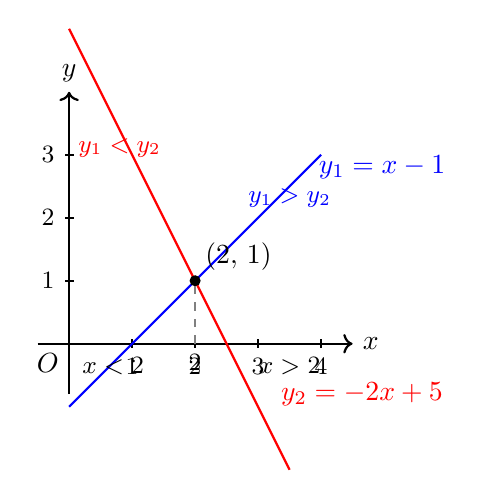
\begin{tikzpicture}[scale=0.8, thick]
  % 坐标轴
  \draw[->] (-0.5,0) -- (4.5,0) node[right] {$x$};
  \draw[->] (0,-0.8) -- (0,4.0) node[above] {$y$};
  \node[below left] at (0,0) {$O$};

  % 刻度
  \foreach \x in {1,2,3,4} {
    \draw (\x, 2pt) -- (\x, -2pt) node[below] {\small$\x$};
  }
  \foreach \y in {1,2,3} {
    \draw (2pt,\y) -- (-2pt,\y) node[left] {\small$\y$};
  }

  % y1 = x - 1（蓝色）
  \draw[blue, thick] (0,-1) -- (4.0, 3.0);
  \node[right, blue] at (3.8, 2.8) {$y_1=x-1$};

  % y2 = -2x + 5（红色）
  \draw[red, thick] (0,5) -- (3.5, -2.0);
  \node[right, red] at (3.2, -0.8) {$y_2=-2x+5$};

  % 交点 (2,1)
  \fill (2,1) circle (2.5pt);
  \node[above right] at (2,1) {$(2,\,1)$};

  % 标注区域
  \draw[gray, dashed] (2,0) -- (2,1);
  \node[below] at (2,0) {\small$2$};

  % 区域标注
  \node[above, blue, font=\small] at (3.5, 2.0) {$y_1>y_2$};
  \node[above, red, font=\small] at (0.8, 2.8) {$y_1<y_2$};
  \node[font=\small] at (3.5,-0.35) {$x>2$};
  \node[font=\small] at (0.7,-0.35) {$x<2$};
\end{tikzpicture}
\end{document}
